\documentclass[aspectratio=169,10pt]{beamer}

\usetheme{metropolis}
\usepackage{appendixnumberbeamer}
\usepackage{booktabs}
\usepackage{amsmath,amssymb}
\usepackage{tikz}
\usetikzlibrary{arrows.meta,positioning,calc,decorations.pathreplacing,shapes.geometric,fit}
\usepackage{pgfplots}
\pgfplotsset{compat=1.18}
\usepackage{xcolor}
\usepackage{colortbl}
\usepackage{multicol}
\usepackage{graphicx}
\usepackage{hyperref}
\hypersetup{colorlinks=true,urlcolor=columbia,linkcolor=columbia}

\definecolor{columbia}{RGB}{29,79,145}
\definecolor{columbialight}{RGB}{117,170,219}
\definecolor{columbiaaccent}{RGB}{210,73,42}
\definecolor{columbiagray}{RGB}{117,117,117}
\definecolor{softbg}{RGB}{245,245,250}
\definecolor{hlgreen}{RGB}{46,139,87}

\setbeamercolor{frametitle}{bg=columbia,fg=white}
\setbeamercolor{progress bar}{fg=columbiaaccent}
\setbeamercolor{alerted text}{fg=columbiaaccent}
\setbeamercolor{block title}{bg=columbia,fg=white}
\setbeamercolor{block body}{bg=softbg}

\setbeamerfont{title}{size=\Large,series=\bfseries}
\setbeamerfont{subtitle}{size=\normalsize}

\graphicspath{{./figures/}}

\title{Lecture 24: Causality and Fairness}
\subtitle{BINF 4002 --- Machine Learning for Health}
\author{Matthew McDermott}
\institute{Dept.\ of Biomedical Informatics, Columbia University}
\date{April 16, 2026}

\begin{document}

\begin{frame}[noframenumbering]
\maketitle
\end{frame}

% ============================================================
\begin{frame}{Where We Are}
\textbf{Course progression:}
\begin{itemize}
    \item[\textcolor{columbiagray}{$\bullet$}] L17--18: EHR \& Claims (confounding introduced)
    \item[\textcolor{columbiagray}{$\bullet$}] L20: Clinical NLP (stigmatizing language, racial bias)
    \item[\textcolor{columbiagray}{$\bullet$}] L23 (Tue): PopHealth --- survival analysis, confounding DAGs, ``are HRs causal?''
    \item[\textcolor{columbiaaccent}{$\to$}] \alert{L24: Causality and Fairness} $\gets$ \textbf{today}
\end{itemize}

\vspace{0.3em}
\textbf{Tuesday (L23):} We saw confounding DAGs, survival analysis, and asked ``are hazard ratios causal?''

\vspace{0.2em}
\textbf{Today, two parts:}
\begin{enumerate}
    \item \textbf{Causality:} What is a causal DAG? How do we estimate causal effects from observational data?
    \item \textbf{Fairness:} What does it mean for a model to be unfair? Why does answering that require causal reasoning?
\end{enumerate}
\end{frame}

% ============================================================
\section{Part I: Causality}
% ============================================================

\begin{frame}{What Is a Causal DAG?}
A \textbf{Directed Acyclic Graph (DAG)} is a model of how variables causally relate.

\vspace{0.3em}
\begin{center}
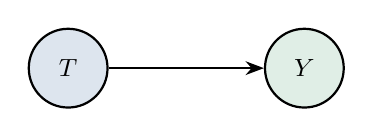
\begin{tikzpicture}[
    var/.style={draw,circle,minimum size=1cm,font=\small,thick},
    >=Stealth
]
\node[var,fill=columbia!15] (x) at (0,0) {$T$};
\node[var,fill=hlgreen!15] (y) at (3,0) {$Y$};
\draw[->,thick] (x) -- (y);
\end{tikzpicture}
\end{center}

\vspace{0.2em}
\begin{itemize}
    \item \textbf{Nodes} $=$ variables (treatment $T$, outcome $Y$, covariates $\mathbf{X}$, \ldots)
    \item \textbf{Edges} $=$ direct causal relationships. $T \to Y$ means ``$T$ is modeled as a direct cause of $Y$''
    \item \textbf{Direction matters.} $T \to Y$ is not the same as $Y \to T$
    \item \textbf{Acyclic:} no directed feedback loops
\end{itemize}

\vspace{0.2em}
{\small Edges encode our \emph{assumptions} about causal structure, based on domain knowledge---not certainties. You've seen DAGs earlier in the course; today we formalize the vocabulary.}
\end{frame}

% ============================================================
\begin{frame}{Prediction vs.\ Intervention: The $do$-Operator}
\textbf{Everything in this course so far:} prediction.
$$P(Y \mid T = 1) \quad\text{--- Among patients who \emph{received} treatment, what is }Y\text{?}$$

\pause
\textbf{The causal question is different:}
$$P(Y \mid do(T = 1)) \quad\text{--- If we \emph{intervene} to assign treatment, what happens to }Y\text{?}$$

\vspace{0.3em}
\textbf{What $do(\cdot)$ means:} We reach into the system and \emph{force} $T$ to a value, breaking all arrows \emph{into} $T$. We no longer condition on who happened to receive treatment---we set it.

\vspace{0.3em}
\textbf{Example:} Patients prescribed drug ($T{=}1$) have lower readmission. But healthier patients are more likely to be prescribed it. So $P(Y|T{=}1) \neq P(Y|do(T{=}1))$---the association overstates the drug's benefit.

\vspace{0.2em}
{\small \textbf{RCTs compute $P(Y|do(T))$ by design.} Randomization breaks arrows into $T$. Can we recover $do(\cdot)$ from observational data?}
\end{frame}

% ============================================================
\begin{frame}{Three DAG Patterns, Three Rules}
\begin{center}
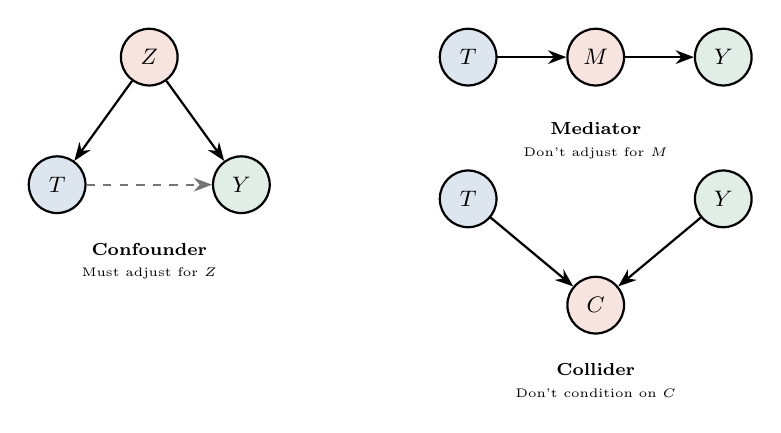
\begin{tikzpicture}[
    var/.style={draw,circle,minimum size=0.8cm,font=\small,thick},
    >=Stealth,
    scale=0.9, transform shape
]
% Confounder
\node[var,fill=columbiaaccent!15] (z1) at (0,1.5) {$Z$};
\node[var,fill=columbia!15] (x1) at (-1.3,-0.3) {$T$};
\node[var,fill=hlgreen!15] (y1) at (1.3,-0.3) {$Y$};
\draw[->,thick] (z1) -- (x1);
\draw[->,thick] (z1) -- (y1);
\draw[->,thick,dashed,columbiagray] (x1) -- (y1);
\node[below=0.0cm,font=\scriptsize\bfseries] at (0,-1.0) {Confounder};
\node[below=0.0cm,font=\tiny] at (0,-1.35) {Must adjust for $Z$};

% Mediator
\node[var,fill=columbia!15] (x2) at (4.5,1.5) {$T$};
\node[var,fill=columbiaaccent!15] (m2) at (6.3,1.5) {$M$};
\node[var,fill=hlgreen!15] (y2) at (8.1,1.5) {$Y$};
\draw[->,thick] (x2) -- (m2);
\draw[->,thick] (m2) -- (y2);
\node[below=0.0cm,font=\scriptsize\bfseries] at (6.3,0.7) {Mediator};
\node[below=0.0cm,font=\tiny] at (6.3,0.35) {Don't adjust for $M$};

% Collider
\node[var,fill=columbia!15] (x3) at (4.5,-0.5) {$T$};
\node[var,fill=hlgreen!15] (y3) at (8.1,-0.5) {$Y$};
\node[var,fill=columbiaaccent!15] (c3) at (6.3,-2.0) {$C$};
\draw[->,thick] (x3) -- (c3);
\draw[->,thick] (y3) -- (c3);
\node[below=0.0cm,font=\scriptsize\bfseries] at (6.3,-2.7) {Collider};
\node[below=0.0cm,font=\tiny] at (6.3,-3.05) {Don't condition on $C$};
\end{tikzpicture}
\end{center}

\vspace{-0.2em}
{\small
\textbf{Confounder:} $Z$ causes both $T$ and $Y$. Failing to adjust $\to$ spurious association.\\
\textbf{Mediator:} $M$ is \emph{on} the causal path. Adjusting blocks the effect you want to measure.\\
\textbf{Collider:} $T$ and $Y$ both cause $C$. Conditioning on $C$ \emph{creates} a spurious association.}
\end{frame}

% ============================================================
\begin{frame}{Exercise: Match the Scenario to the DAG}
\textbf{For each DAG, assign the real-world variables to the nodes.}

\vspace{0.3em}
\begin{columns}[T]
\column{0.48\textwidth}
\textbf{1.} \; $Z \to T$, \; $Z \to Y$\\ {\scriptsize (confounder)}\\[0.3em]
Variables: \emph{ice cream sales}, \emph{drowning deaths}, \emph{summer temperature}

\vspace{0.5em}
\textbf{2.} \; $T \to C \leftarrow Y$\\ {\scriptsize (collider)}\\[0.3em]
Variables: \emph{respiratory disease}, \emph{bone fractures}, \emph{hospitalization}

\column{0.48\textwidth}
\textbf{3.} \; $T \to M \to Y$\\ {\scriptsize (mediator)}\\[0.3em]
Variables: \emph{smoking}, \emph{tar deposits in lungs}, \emph{lung cancer}

\vspace{0.5em}
\textbf{4.} \; $Z \to T$, \; $Z \to Y$\\ {\scriptsize (confounder)}\\[0.3em]
Variables: \emph{treatment choice}, \emph{recovery rate}, \emph{disease severity}
\end{columns}

\vspace{0.5em}
\pause
{\small \textbf{Key question for each:} Should you adjust for the middle variable? Why or why not?}
\end{frame}

% ============================================================
\begin{frame}{A Gallery of Biases}
Each bias you've seen this semester is a DAG pattern:

\vspace{0.2em}
\begin{center}
\renewcommand{\arraystretch}{1.2}
{\footnotesize
\begin{tabular}{p{2cm}p{2.5cm}p{7cm}}
\toprule
\textbf{DAG pattern} & \textbf{Named bias} & \textbf{Health example} \\
\midrule
Confounder & Simpson's Paradox & Stone size $\to$ treatment + outcome. Aggregate reverses stratified. \\
Collider & Berkson's paradox & Resp.\ disease + fracture both $\to$ hospitalization. Spurious negative correlation. \\
Collider & Healthy volunteer & Health + motivation both $\to$ enrollment. Volunteers are systematically different. \\
Mediator & Overadjustment & Treatment $\to$ BP $\to$ outcome. Adjusting for BP blocks the treatment effect. \\
\bottomrule
\end{tabular}
}
\end{center}

\vspace{0.1em}
{\small [Next slide: each pattern's data consequence]}
\end{frame}

% ============================================================
\begin{frame}{Gallery of Biases}
\centering
\includegraphics[width=\textwidth,height=0.75\textheight,keepaspectratio]{fig1_bias_gallery.png}

\vspace{-0.3em}
{\scriptsize Four named biases, four DAG patterns. Each panel: the causal structure on the left, the data consequence on the right. (Charig et al.\ 1986; Fry et al.\ 2017.)}
\end{frame}

% ============================================================
\begin{frame}{Propensity Score Methods}
\begin{columns}[T]
\column{0.70\textwidth}
\textbf{Intuition:} If two patients are identical in covariates but one got treatment ($T{=}1$) and one didn't ($T{=}0$), their outcome difference estimates a causal effect. But ``identical'' is impractical. We only need them equally \emph{likely} to receive treatment.

\vspace{0.3em}
\textbf{Propensity score:} $e(\mathbf{X}) = P(T{=}1 \mid \mathbf{X})$\\
{\scriptsize ($\mathbf{X}$ = full covariate vector; $Z$ in the earlier DAGs was a single confounder)}

\vspace{0.2em}
\textbf{Three uses:}
\begin{itemize}
    \item \textbf{Matching:} pair treated/untreated with similar $e(\mathbf{X})$
    \item \textbf{IPTW:} weight by $1/e(\mathbf{X})$ or $1/(1{-}e(\mathbf{X}))$
    \item \textbf{Stratification:} estimate within PS quantiles
\end{itemize}

\column{0.27\textwidth}
\begin{center}
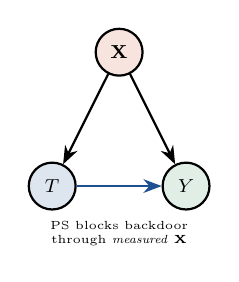
\begin{tikzpicture}[
    var/.style={draw,circle,minimum size=0.7cm,font=\footnotesize,thick},
    >=Stealth,
    scale=0.85, transform shape
]
\node[var,fill=columbiaaccent!15] (z) at (1,2) {$\mathbf{X}$};
\node[var,fill=columbia!15] (x) at (0,0) {$T$};
\node[var,fill=hlgreen!15] (y) at (2,0) {$Y$};
\draw[->,thick] (z) -- (x);
\draw[->,thick] (z) -- (y);
\draw[->,thick,columbia] (x) -- (y);
\node[below=0.1cm,font=\tiny,align=center] at (1,-0.3) {PS blocks backdoor\\through \emph{measured} $\mathbf{X}$};
\end{tikzpicture}
\end{center}
\end{columns}

\vspace{0.2em}
{\small \textbf{Assumptions:} no unmeasured confounders (untestable) + overlap/positivity. In practice, always check \textbf{balance diagnostics}: do covariate distributions look similar after matching/weighting?}

{\small [Notebook Fig.~2: real NHEFS data]}
\end{frame}

% ============================================================
\begin{frame}{Propensity Score: Real Data (Notebook Fig.~2)}
\centering
\includegraphics[width=\textwidth,height=0.68\textheight,keepaspectratio]{fig2_propensity_scores.png}

\vspace{-0.3em}
{\scriptsize Real NHEFS data (Hern\'an \& Robins). Does quitting smoking ($T{=}1$) cause weight gain? Na\"{\i}ve: 2.5~kg (confounded). IPTW: 3.3~kg---matching the published $\sim$3.4~kg.}
\end{frame}

% ============================================================
\begin{frame}{Challenges in Causal Inference}
If causal inference is so useful, why isn't everything causal?

\vspace{0.3em}
\begin{itemize}[<+->]
    \item \textbf{Unmeasured confounding.} The no-unmeasured-confounders assumption is \emph{untestable}. If a key variable is missing from the data, PS methods silently give the wrong answer.
    \item \textbf{Time-varying treatments.} A patient's treatment at month 3 depends on their outcome at month 2. Standard PS breaks down; need marginal structural models or g-computation.
    \item \textbf{Transportability.} A causal effect estimated in one population may not hold in another (different confounders, different effect modifiers).
    \item \textbf{Interference.} One patient's treatment affects another's outcome (vaccination, infection control). Violates the stable unit treatment value assumption (SUTVA).
\end{itemize}

\vspace{0.2em}
\onslide<5->{{\small Sensitivity analyses help: ``how strong would an unmeasured confounder need to be to explain away the result?''}}
\end{frame}

% ============================================================
\section{Part II: Fairness}
% ============================================================

\begin{frame}{What Does It Mean to Be Unfair?}
Your hospital deploys a risk score $\hat{R} = f(\mathbf{X}) \in [0,1]$ to flag patients for follow-up. Two groups (defined by a protected attribute $A$) have different error rates.

\vspace{0.5em}
\textbf{Clinician A says:} ``A score of 30\% means 30\% regardless of group. That's fair.''

\vspace{0.3em}
\textbf{Clinician B says:} ``Among patients who actually had the event, the model missed more in one group. That's unfair.''

\vspace{0.5em}
\pause
Both are reasonable. Both are precise. \alert{They cannot both be satisfied.}

\vspace{0.3em}
{\small \textbf{Notation:} $Y \in \{0,1\}$ is the true outcome, $A$ is the protected attribute, $\hat{R} = f(\mathbf{X}) \in [0,1]$ is the model's predicted probability (a random variable because it depends on the random covariates $\mathbf{X}$).}
\end{frame}

% ============================================================
\begin{frame}{Two Definitions: Sufficiency and Separation}

\vspace{0.3em}
\begin{center}
\renewcommand{\arraystretch}{1.4}
{\small
\begin{tabular}{lll}
\toprule
\textbf{Property} & \textbf{Formal} & \textbf{Meaning} \\
\midrule
\textbf{Sufficiency} {\scriptsize (calibration)} & $Y \perp A \mid \hat{R}$ & The score means the same thing for everyone. \\
\textbf{Separation} {\scriptsize (equalized errors)} & $\hat{R} \perp A \mid Y$ & Equal TPR and FPR across groups. \\
\bottomrule
\end{tabular}
}
\end{center}

\vspace{0.3em}
\pause
Both are \textbf{conditional independence} properties.\\
\textbf{Sufficiency} $=$ Clinician A's intuition. \textbf{Separation} $=$ Clinician B's.

\vspace{0.3em}
{\small \textbf{Note:} $\hat{R}$ is a predicted probability, not a binary decision. When we threshold $\hat{R}$ to make a decision, sufficiency becomes a property of how the score relates to outcomes; separation becomes a property of error rates.}
\end{frame}

% ============================================================
\begin{frame}{Worked Example: Sufficiency vs.\ Separation}
\textbf{200 pts/group. Two risk bins. Flag the \colorbox{hlgreen!12}{High} column.}

\vspace{0.1em}
\begin{center}
{\scriptsize
\renewcommand{\arraystretch}{1.15}
\begin{tabular}{l >{\columncolor{columbiagray!8}}c >{\columncolor{hlgreen!12}}c}
\toprule
& $\hat{R} = \text{Low}$ (0.2) & $\hat{R} = \text{High}$ (0.8) \\
\midrule
\textbf{Group A} (prev 50\%) & 100 pts: \textcolor{columbiaaccent}{20 ill}, \textcolor{columbia}{80 well} & 100 pts: \textcolor{columbiaaccent}{80 ill}, \textcolor{columbia}{20 well} \\
\textbf{Group B} (prev 35\%) & 150 pts: \textcolor{columbiaaccent}{30 ill}, \textcolor{columbia}{120 well} & 50 pts: \textcolor{columbiaaccent}{40 ill}, \textcolor{columbia}{10 well} \\
\midrule
\textbf{Calibration} & $20\%$ \checkmark \; same both & $80\%$ \checkmark \; same both \\
\bottomrule
\end{tabular}
}
\end{center}

\vspace{-0.1em}
{\small \textbf{Sufficiency holds (by construction):} score of 0.2 means 20\% \textcolor{columbiaaccent}{ill} regardless of group. $\checkmark$}

\pause
\vspace{0.1em}
{\scriptsize
\textbf{TPR} $= \tfrac{\colorbox{hlgreen!12}{\textcolor{columbiaaccent}{ill, High}}}{\colorbox{hlgreen!12}{\textcolor{columbiaaccent}{ill, High}} + \colorbox{columbiagray!10}{\textcolor{columbiaaccent}{ill, Low}}}$
\quad
A: $\tfrac{\colorbox{hlgreen!12}{\textcolor{columbiaaccent}{80}}}{\colorbox{hlgreen!12}{\textcolor{columbiaaccent}{80}} + \colorbox{columbiagray!12}{\textcolor{columbiaaccent}{20}}} = 80\%$
\quad
B: $\tfrac{\colorbox{hlgreen!12}{\textcolor{columbiaaccent}{40}}}{\colorbox{hlgreen!12}{\textcolor{columbiaaccent}{40}} + \colorbox{columbiagray!12}{\textcolor{columbiaaccent}{30}}} = 57\%$

\vspace{0.15em}
\textbf{FPR} $= \tfrac{\colorbox{hlgreen!12}{\textcolor{columbia}{well, High}}}{\colorbox{hlgreen!12}{\textcolor{columbia}{well, High}} + \colorbox{columbiagray!10}{\textcolor{columbia}{well, Low}}}$
\quad
A: $\tfrac{\colorbox{hlgreen!12}{\textcolor{columbia}{20}}}{\colorbox{hlgreen!12}{\textcolor{columbia}{20}} + \colorbox{columbiagray!12}{\textcolor{columbia}{80}}} = 20\%$
\quad
B: $\tfrac{\colorbox{hlgreen!12}{\textcolor{columbia}{10}}}{\colorbox{hlgreen!12}{\textcolor{columbia}{10}} + \colorbox{columbiagray!12}{\textcolor{columbia}{120}}} = 8\%$
}

\vspace{0.1em}
\alert{Both differ $\to$ separation fails.}
\pause
{\small \; To equalize: lower threshold for B $\to$ same score, different action for different groups.}
\end{frame}

% ============================================================
\begin{frame}{The Impossibility Theorem (Chouldechova 2017)}
\textbf{Theorem.} If prevalence differs between groups ($P(Y{=}1|A{=}a) \neq P(Y{=}1|A{=}b)$), then sufficiency and separation are \textbf{mutually incompatible} for any risk score that makes errors (i.e., $\text{TPR} < 1$ or $\text{FPR} > 0$).

\vspace{0.5em}
\pause
\textbf{Intuition:} If the base rate differs, a calibrated score must assign different score distributions to each group. But then error rates \emph{cannot} be equal.

\vspace{0.5em}
\begin{block}{Why this matters}
In health, prevalence almost always differs by demographics. Fairness requires \textbf{human choices} about which property to prioritize.
\end{block}

{\small \textbf{Connection to L23:} If you are predicting a conditional outcome (e.g., readmission given survival to discharge), the conditioning event itself may differ across groups---adding another layer to the fairness problem.}
\end{frame}

% ============================================================
\begin{frame}{Impossibility in Practice (Notebook Fig.~3)}
\centering
\includegraphics[width=\textwidth,height=0.68\textheight,keepaspectratio]{fig3_impossibility.png}

\vspace{-0.3em}
{\scriptsize MEPS data. Left: calibration curves approximately on the diagonal---\textbf{close to sufficiency}. Middle: TPR/FPR differ---\textbf{separation fails}. Right: to equalize TPR, use a lower threshold for Non-White. The gold zone shows scores where one group is flagged but the other is not---same score, different decision.}
\end{frame}

% ============================================================
\begin{frame}{From Metric Fairness to Causal Fairness}
A natural fairness question:

\vspace{0.3em}
\begin{block}{}
\emph{If nothing changed about a patient but their race, would the risk score change?}
\end{block}

\vspace{0.3em}
\pause
This seems simple---but it is actually a \textbf{causal} question. It asks about an intervention: $do(A = a')$.

\vspace{0.3em}
And race is not a simple variable you can $do()$ on. It is entangled with access, environment, provider behavior, measurement quality.

\vspace{0.3em}
\pause
\textbf{The better question:} Which causal \emph{pathways} from $A$ into $\hat{R}$ are legitimate, and which reflect structural bias? To answer this, we need a DAG.
\end{frame}

% ============================================================
\begin{frame}{Obermeyer et al.\ (2019): The Canonical Case Study}
A widely-deployed algorithm determined which patients were referred to high-risk care management.

\vspace{0.3em}
\textbf{The problem:}
\begin{itemize}[<+->]
    \item The algorithm predicted \textbf{healthcare cost} as a proxy for healthcare \textbf{need}
    \item At the same level of true illness, Black patients had \textbf{lower costs}
    \item Why? Differential access, trust, historical underinvestment
    \item Result: Black patients had to be \textbf{sicker} to receive the same risk score
    \item Correcting this would increase Black patients referred from 17.7\% to 46.5\%
\end{itemize}
\end{frame}

% ============================================================
\begin{frame}{Obermeyer: The Mechanism (as a DAG)}
\begin{center}
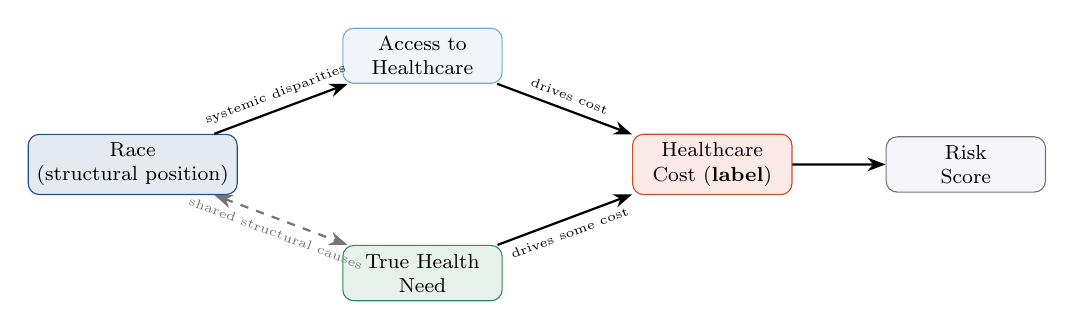
\begin{tikzpicture}[
    box/.style={draw,rounded corners,minimum width=2.2cm,minimum height=0.65cm,align=center,font=\footnotesize},
    >=Stealth,
    scale=0.92, transform shape
]
\node[box,fill=columbia!12,draw=columbia] (race) at (0,1) {Race\\(structural position)};
\node[box,fill=columbia!6,draw=columbialight] (access) at (4,2.5) {Access to\\Healthcare};
\node[box,fill=hlgreen!12,draw=hlgreen] (need) at (4,-0.5) {True Health\\Need};
\node[box,fill=columbiaaccent!12,draw=columbiaaccent] (cost) at (8,1) {Healthcare\\Cost (\textbf{label})};
\node[box,fill=softbg,draw=columbiagray] (model) at (11.5,1) {Risk\\Score};

\draw[->,thick] (race) -- (access) node[midway,above,font=\tiny,sloped] {systemic disparities};
\draw[->,thick] (access) -- (cost) node[midway,above,font=\tiny,sloped] {drives cost};
\draw[{Stealth}-{Stealth},thick,dashed,columbiagray] (race) -- (need) node[midway,below,font=\tiny,sloped] {shared structural causes};
\draw[->,thick] (need) -- (cost) node[midway,below,font=\tiny,sloped] {drives some cost};
\draw[->,thick] (cost) -- (model);
\end{tikzpicture}
\end{center}

\vspace{0.2em}
{\small \textbf{Bias path:} Race $\to$ Access $\to$ Cost $\to$ Score. The bidirected arrow ($\leftrightarrow$) between Race and Need means they share unmeasured common causes (environment, historical disinvestment)---not that race directly causes disease. The fix: predict Need directly.}
\end{frame}

% ============================================================
\begin{frame}{Obermeyer Replication (Notebook Fig.~4)}
\centering
\includegraphics[width=\textwidth,height=0.68\textheight,keepaspectratio]{fig4_obermeyer.png}

\vspace{-0.3em}
{\scriptsize Data from the authors' published synthpop dataset. At the same algorithm risk score, Black patients have substantially more active chronic conditions. The algorithm systematically under-refers Black patients.}
\end{frame}

% ============================================================
\begin{frame}{Causal Fairness}
\begin{block}{The causal fairness question}
\textbf{Which causal pathways} from a protected attribute $A$ into the prediction $\hat{R}$ are we willing to treat as \textbf{legitimate}, and which reflect \textbf{structural bias}?
\end{block}

\vspace{0.2em}
In the Obermeyer DAG:
\begin{itemize}[<+->]
    \item $A \to \text{Access} \to \text{Cost} \to \hat{R}$: reflects \textbf{unjust structure}
    \item $A \leftrightarrow \text{Need}$: shared structural causes. Routing through \emph{clinical need} rather than cost avoids the inequitable pathway
\end{itemize}

\vspace{0.2em}
\onslide<3->{\textbf{Causal fairness is not about ``changing race.''} It is about which \emph{pathways} a prediction should be allowed to travel.}

\vspace{0.1em}
\onslide<3->{{\scriptsize \textbf{Going further:} \emph{Principal fairness} (Imai \& Jiang 2023) defines fairness via potential outcomes---individuals who would benefit equally from treatment should be treated equally, regardless of group.}}
\end{frame}

% ============================================================
\begin{frame}{Subgroup Evaluation: The Minimum Standard}
\textbf{Aggregate metrics hide disparities.}

\vspace{0.3em}
\textbf{Minimum practice:} Stratified reporting by protected attributes.
\begin{itemize}
    \item AUC, sensitivity, PPV---\emph{per group}
    \item Confidence intervals or bootstrap error bars
    \item Report the \textbf{gap}, not just the group values
\end{itemize}

\vspace{0.3em}
\textbf{Why models fail subgroups:}
\begin{enumerate}
    \item Underrepresentation in training data
    \item Different feature distributions across groups
    \item Different label quality across groups (recall Obermeyer)
\end{enumerate}

{\small [Notebook Fig.~5: MEPS healthcare utilization---analogous to clinical risk scores]}
\end{frame}

% ============================================================
\begin{frame}{Subgroup Performance (Notebook Fig.~5)}
\centering
\includegraphics[width=\textwidth,height=0.68\textheight,keepaspectratio]{fig5_subgroup_eval.png}

\vspace{-0.3em}
{\scriptsize MEPS healthcare utilization. Left: absolute metrics by group. Right: the gap (White $-$ Non-White). \textbf{Gaps reverse direction across metrics}---no group is uniformly advantaged. This is why stratified reporting is the minimum standard.}
\end{frame}

% ============================================================
\begin{frame}{Mitigation: Three Intervention Points}
\begin{center}
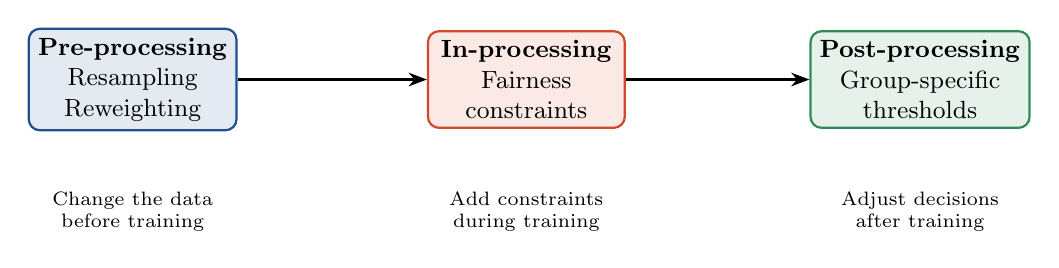
\begin{tikzpicture}[
    stage/.style={draw,thick,rounded corners,minimum width=2.5cm,minimum height=1cm,align=center,font=\small},
    >=Stealth
]
\node[stage,fill=columbia!12,draw=columbia] (pre) at (0,0) {\textbf{Pre-processing}\\Resampling\\Reweighting};
\node[stage,fill=columbiaaccent!12,draw=columbiaaccent] (in) at (5,0) {\textbf{In-processing}\\Fairness\\constraints};
\node[stage,fill=hlgreen!12,draw=hlgreen] (post) at (10,0) {\textbf{Post-processing}\\Group-specific\\thresholds};

\draw[->,thick] (pre) -- (in);
\draw[->,thick] (in) -- (post);

\node[below=0.5cm,font=\scriptsize,align=center] at (0,-0.8) {Change the data\\before training};
\node[below=0.5cm,font=\scriptsize,align=center] at (5,-0.8) {Add constraints\\during training};
\node[below=0.5cm,font=\scriptsize,align=center] at (10,-0.8) {Adjust decisions\\after training};
\end{tikzpicture}
\end{center}

\vspace{0.3em}
Each trades one fairness property for another. \textbf{No free lunch}---recall the impossibility theorem.

\vspace{0.2em}
\textbf{Complication:} Group-specific thresholds require knowing group membership at inference time. Whether using $A$ in a clinical algorithm is legal---even to improve fairness---is an active policy debate.

{\small [Notebook Fig.~6: before/after threshold adjustment]}
\end{frame}

% ============================================================
\begin{frame}{Threshold Adjustment (Notebook Fig.~6)}
\centering
\includegraphics[width=\textwidth,height=0.68\textheight,keepaspectratio]{fig6_threshold_adjustment.png}

\vspace{-0.3em}
{\scriptsize Left: default threshold yields unequal TPR. Right: group-specific thresholds equalize TPR, but FPR and PPV diverge. Equalizing one error-rate metric forces others apart.}
\end{frame}

% ============================================================
\section{Synthesis}
% ============================================================

\begin{frame}{Practical Scenario}
\textbf{A readmission risk model at your hospital.}

\vspace{0.2em}
\begin{enumerate}[<+->]
    \item The model outputs $\hat{R} \in [0,1]$ with AUC 0.82 overall. Do you ship it?
    \item You check subgroups: AUC is 0.86 for White patients, 0.74 for Black patients.
    \item The label is ``readmitted within 30 days''---but readmission is an imperfect proxy for deterioration (access affects whether worsening is captured). Is the label biased?
    \item You equalize TPR across groups. PPV diverges. Sufficiency or separation?
    \item Insurance type confounds both readmission and follow-up access. Draw the DAG. What causal method might help?
\end{enumerate}
\end{frame}

% ============================================================
\begin{frame}{Summary}
\begin{center}
\renewcommand{\arraystretch}{1.2}
{\footnotesize
\begin{tabular}{lp{7.5cm}}
\toprule
\textbf{Concept} & \textbf{Key takeaway} \\
\midrule
Causal DAGs & Nodes $=$ variables, edges $=$ modeled direct causes. Confounder: adjust. Mediator: don't. Collider: don't condition. \\
$P(Y|T)$ vs.\ $P(Y|do(T))$ & Prediction $\neq$ causation. $do(\cdot)$ breaks arrows into $T$. \\
Propensity scores & $e(\mathbf{X}) = P(T{=}1|\mathbf{X})$. Requires no unmeasured confounders + overlap. \\
Sufficiency vs.\ separation & $Y \perp A | \hat{R}$ vs.\ $\hat{R} \perp A | Y$; incompatible when prevalence differs. \\
Label bias & Most dangerous bias is in the label, not the model (Obermeyer). \\
Causal fairness & Which pathways from $A$ into $\hat{R}$ are legitimate? \\
\bottomrule
\end{tabular}
}
\end{center}
\end{frame}

% ============================================================
\begin{frame}[standout]
    Questions?
\end{frame}

% ============================================================
\appendix
% ============================================================

\begin{frame}{Appendix: Where Is Causal Inference Going?}
\begin{itemize}
    \item \textbf{Targeted learning (TMLE):} ML for nuisance parameters + semiparametric efficiency. Doubly robust.
    \item \textbf{Double/debiased ML:} ML confounding adjustment with valid inference (Chernozhukov et al.\ 2018).
    \item \textbf{Causal forests:} Heterogeneous treatment effects---which subgroups benefit most? (Athey \& Imbens 2016).
    \item \textbf{Causal reasoning with foundation models:} Can LLMs help with causal graph construction? Active research.
\end{itemize}

\vspace{0.3em}
{\small \textbf{Key reference:} Hern\'an \& Robins, \emph{Causal Inference: What If} (freely available online). The NHEFS dataset we used is from this textbook.}
\end{frame}

\end{document}
